The \ac{ROI} is a typical financial performance measure to evaluate the efficiency of an investment. To be able to analyze any hypothetical investments, a market analysis should be performed indicating possible organizations, companies or individuals (which are from now on referred to as 'users') that might be interested in the delivered product, service or data. Considering that any mission is specifically user-demanded, the option to attract several users from multiple scientific fields is limited. However, regarding the high price per kilogram (\$4,000 - \$40,000 / kg depending on launcher and altitude) to put in Earth orbit, it probably would not suffice to have a positive return on \acs{ROI} using a small amount of users. 

It should be noted that the \acs{ROI} is usually mistakenly misinterpreted by considering the potential financial profit only. The term 'return' does not state financial return implicitly. Of course, increasing the potential financial profit increases the feasibility of the mission. Nevertheless, the return can also refer to scientific or educational gain, which can be seen as long term \acs{ROI}. 

\section{Market Analyses}
  \label{blMAanalyses}
The market analysis determines the main potential users and is mainly dependent on the quality and quantity of the obtained data. There are four types of the measurement data sets and it is convenient to analyze them separately. Figure \ref{MA} on page \pageref{MA} gives the market diagram with different data sets.
\begin{figure} [h]
	\begin{center}
 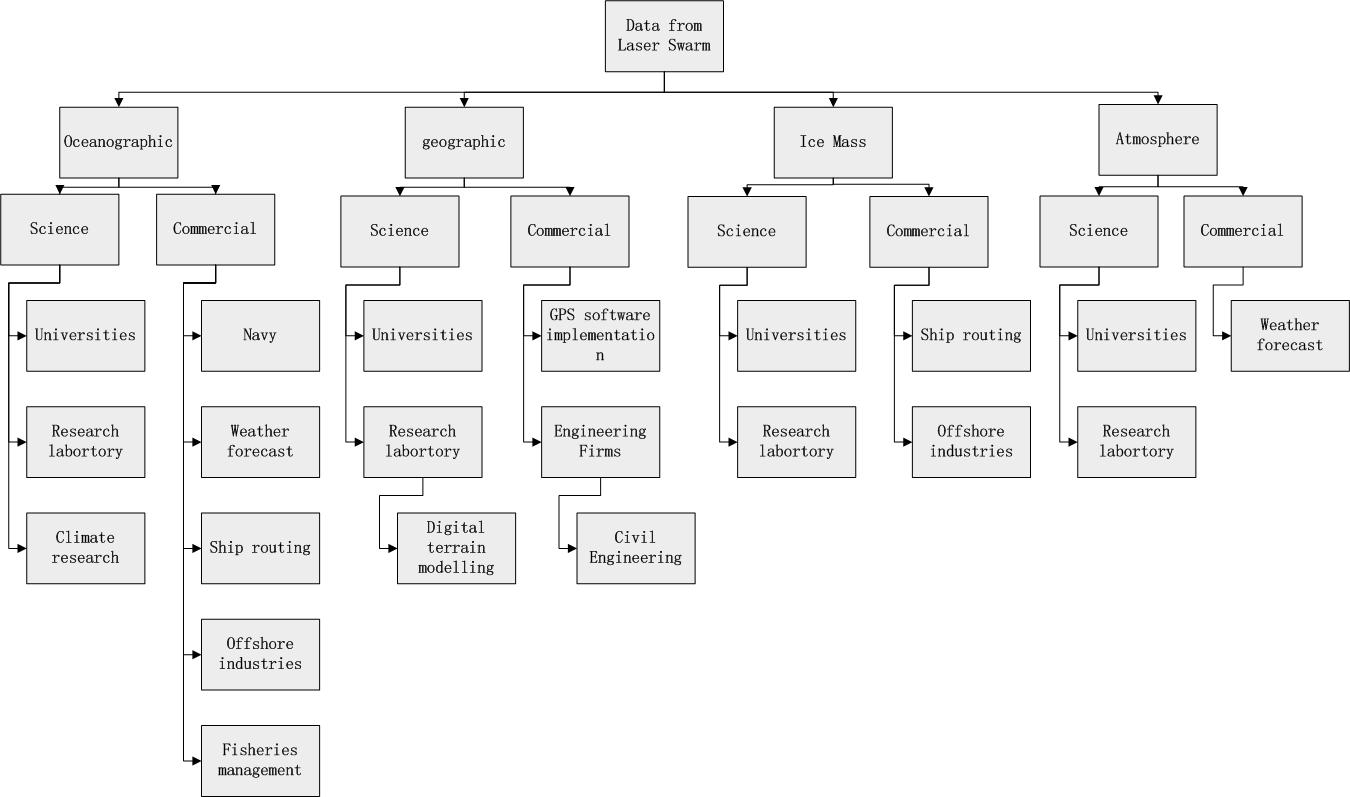
\includegraphics[width=0.85\textwidth,angle=0]{chapters/img/Market_analysis.jpg}	
	\caption{Market Breakdown Diagram with different data sets\cite{Market}}
	\label{MA}
	\end{center}
\end{figure}
In the Market Breakdown Diagram, each data type has both science and commercial potential users. For example in science field, the oceanographic data can be used for climate research. Scientist can study the evolution of weather patterns from the ocean system by modeling changes in the distribution of heat in the ocean. On the other hand in commercial field, maps of current, eddies and vector winds are used in commercial shipping and recreational yachting to optimize routes. All the blocks in the diagram could be potential \acs{ROI} on short or long term.

\section{Investment and Profit Opportunities}
	\label{blMAipo}
Short term investments, in this case the investments to cover the preliminary costs as well as the cost for \acs{IAT}, all the subsystems and the implementation of the spacecraft in its orbit, could be determined with a high accuracy, since they are non-recurring. Long term investments are communication with the satellite (constellation), personnel costs and ground station maintenance, and can be considered recurring (with a certain uncertainty). Since the risk of partial failure is severe in any space mission, the quality or the quantity of the data sets can decrease, lowering the \acs{ROI} over time. 

Depending on the actual operational lifetime of the satellite constellation (and especially, the lifetime of the emitter), the data volume over the years can generate a positive \acs{ROI}. If the lifetime of the total system exceeds the determined lifetime upfront, the profit opportunities increase due to an increase in data volume. 

Next to that, a successful space mission could generate trust by users for future missions, which will, on its turn, be more eager to invest in long term projects.

Techniques like \acs{LiDAR} are usually more attractive to the scientific community. In that sense, the potential financial profit is not that important. The \acs{laser} altimetry mission is probably interesting for scientific organizations, like universities and research institutes. The \acs{ROI} is then referred to as return in knowledge.  